\paragraph{Transformers} \label{sec:transformers}

In 2017, the introduction of the ``Attention is All You Need''~\cite{vaswani_attention_2017} paper marked a significant milestone in \ac{DL}. Although initially introduced for \ac{NLP}, the transformer architecture has proven helpful in various data generation tasks, including audio synthesis as shown in Section~\ref{sec:related-work}. This marked a paradigm shift from the conventional \ac{RNN}-based models, which were earlier widely used, with some incorporating a rudimentary form of the attention mechanism.

In transformers, attention is a key component that allows the model to focus on relevant parts of the input sequence when making predictions. Mathematically, attention can be defined as a weighted sum of values based on their importance or relevance.

Let's break down the mathematical formulation of attention in transformers:

Query \(Q\), Key \(K\), and Value \(V\): These are three linear transformations applied to the input sequence. The query represents the element for which we want to compute attention weights, while keys and values represent all elements in the sequence.

To calculate how much each value contributes to the output for a given query, we compute dot products between the query and all keys:

\begin{equation}
    \text{{scores}} = Q \cdot K^T
\end{equation}

Here, \(\cdot\) represents matrix multiplication, \(K^T\) denotes transpose of matrix \(K\).

The next step is to normalize these scores using a softmax function along dimension 1 (rows) to obtain attention weights that sum up to 1:

\begin{equation}
    \text{{weights}} = \text{{softmax}}(\text{{scores}})
\end{equation}

Finally, we take a weighted sum of values using these normalized attention weights:

\begin{equation}
\begin{split}
    &\text{{attended\_values}} = V \cdot {\text{{weights}}} \\
    &\text{{output}} = {\sum{( {\text{attended\_values} } })}
\end{split}
\end{equation}

Here, $\text{softmax}$ computes exponentiated values scaled by their row-wise sums, while $\text{sum}$ performs summation across rows.

The resulting output represents an attended representation obtained by giving higher weightage/importance to more relevant parts of the input sequence based on similarity with respect to the query. This mathematical formulation allows transformer models to capture long-range dependencies effectively by attending to the pertinent information in the source sequence when generating predictions.

The attention mechanism allows the model to give different importance to different input parts. For instance, let us imagine a translation task English-Portuguese. If naively translated, the sentence ``She is a doctor'' could be translated to ``Ela é um doutor''. However, if, when generating the last word, the model gives some importance to the word ``she'', it might guess that the correct word is ``doutora''.

The key idea behind transformers is to completely disregard the recurrent architecture and only use attention by using self-attention. Self-attention is a mechanism that allows the calculation of the importance of each input element concerning all other elements in the input sequence. This allows the model to dynamically focus on the most relevant information at each step of the calculation instead of relying on fixed relationships between elements in the input as in traditional recurrent neural networks.


%% HERE
The transformer architecture, shown in Figure \ref{fig:transformer}, serves as the basis for advanced transformers utilized in a variety of applications, such as audio synthesis. This architecture includes an encoder and decoder, both with stacked layers, which are essential to processing textual input data and producing consistent audio waveforms.

The encoder, consisting of $N$ identical layers, aims to convert the input text into continuous representations that encapsulate crucial semantic information. Each layer features two sub-layers that enable this conversion:

\begin{enumerate}
    \item Multi-Head Self-Attention: As explained above, this mechanism allows the encoder to model input text sequence dependencies objectively. Multiple scaled dot-product attention heads attend to various positions of the text sequence simultaneously. This process captures intricate relationships within the text in parallel, enriching the representation.
    \item Position-wise Feedforward Network: Composed of two linear transformations with \ac{ReLU} activation, this neural network introduces non-linear interactions within the embedded space. These interactions bolster the model's capability to comprehend intricate semantic nuances that exist within the text.
\end{enumerate}

Residual skip connections and layer normalization surround each sub-layer, enhancing training stability. By mapping input text to continuous representations, the encoder empowers subsequent stages to generate audio that aligns with the input's semantics.

The decoder, which includes $M$ stacked layers, generates the output audio waveform while conditioned on the continuous representations from the encoder. This conditioning guarantees that the synthesized audio aligns with the intended semantics of the input text. Each decoder layer comprises three sub-layers.

\begin{enumerate}
    \item Masked Multi-Head Self-Attention over Previous Outputs: This sublayer enables modeling of dependencies between previously generated audio samples, facilitating the creation of coherent output samples. It blocks leftward information flow, ensuring a causal relationship between created samples.

    \item Multi-Head Attention over Encoder Outputs: By attending over the final encoder representations, this sublayer allows the decoder to incorporate the input text semantics into the generation process. This attention mechanism guarantees that the synthesized sample remains aligned with the intended meaning of the input.

    \item The Position-wise Feedforward Network consists of two linear transformations with \ac{ReLU} activation, similar to the encoder. It improves the decoder's ability to comprehend complex relationships between different samples.
\end{enumerate}

Like the encoder, the decoder employs residual connections and layer normalization for stability during training. The decoder generates the output sequentially, predicting one sample at a time. The integration of multi-head attention mechanisms at both the local and global levels enables the synthesis of diverse and natural outputs. This autoregressive process, conditioned on powerful semantic representations, produces high-fidelity outputs aligned with the input.

This architectural change significantly accelerates the training and inference processes by allowing the use of larger data sets while greatly improving the generation results - thus revolutionizing the progress made in the field.

\begin{figure}[ht]
    \centering
    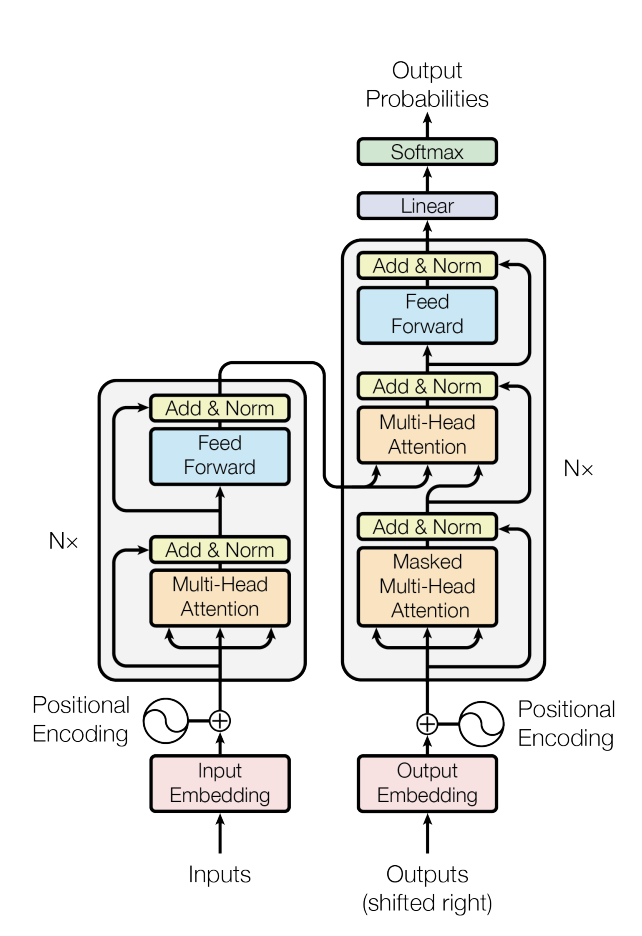
\includegraphics[width=0.5\textwidth, scale=0.8]{figures/2-sota/transformer.png}
    \caption[Transformer]{\textbf{Transformer} --- This illustration was taken from \cite{vaswani_attention_2017} and shows the general architecture of the base transformer. One can see that the constituents are pretty simple. These are simple word embeddings (which are not covered in this study), self-attention, and feedforward layers. The left side of the structure is called the encoder, while the right side is called the decoder.}
    \label{fig:transformer}
\end{figure}